\documentclass[11pt, twocolumn]{article}

\usepackage[spanish]{babel}
\usepackage[none]{hyphenat}
\usepackage[left=1.5cm, right=1.5cm, top = 2cm, bottom=2.5cm]{geometry}
\usepackage{parskip}
\usepackage[export]{adjustbox}
\usepackage{enumitem}
\usepackage{listings}
\usepackage{color}
\usepackage{fancyhdr}
\usepackage{graphicx}
\usepackage{caption}
% \usepackage{subcaption}
% \usepackage{wrapfig}
% \usepackage{longtable}
% \usepackage{multirow, makecell}
% \usepackage{amsmath} 
\usepackage[hidelinks]{hyperref}
\usepackage{csquotes}

\newcommand{\linejump}{\hfill \break}
\renewcommand{\thefootnote}{\fnsymbol{footnote}}
% \newcommand{\unit}[1]{\ensuremath{\, \mathrm{#1}}}

\definecolor{dkgreen}{rgb}{0,0.6,0}
\definecolor{gray}{rgb}{0.5,0.5,0.5}
\definecolor{mauve}{rgb}{0.58,0,0.82}
\lstset{
  language=Java,
  aboveskip=3mm,
  belowskip=3mm,
  showstringspaces=false,
  columns=flexible,
  basicstyle={\tiny\ttfamily},
  numbers=none,
  numberstyle=\tiny\color{gray},
  keywordstyle=\color{blue},
  commentstyle=\color{dkgreen},
  stringstyle=\color{mauve},
  breaklines=true,
  breakatwhitespace=true,
  tabsize=2
}

\sloppy
\setlength{\parindent}{0cm}
\setlength{\columnsep}{0.5cm}
\decimalpoint
\graphicspath{{img/}}

\hypersetup{colorlinks=true, urlcolor=blue, citecolor=blue}
\urlstyle{same}

\pagestyle{fancyplain}
\fancyhf{}
\fancyhead[L]{\scriptsize 
  Universidad Nacional Autónoma de México \\
  Laboratorio de Programación Orientada a Objetos \\
  M.C. Leonardo Ledesma Dominguez
}
\fancyhead[R]{\thepage}


\begin{document}
  \twocolumn[
    \centering
    Acosta Porcayo Alan Omar, Gutiérrez Grimaldo Alejandro, Medina Villa Samuel

    \linejump

    \LARGE \textbf{Práctica 4. Clases y Objetos } \\
    
    \linejump
  ]
      
  \footnotetext{
    \scriptsize 
    Acosta Porcayo Alan Omar Ing. en Computación 320206102 \\
    Gutiérrez Grimaldo Alejandro Ing. en Computación 320282098 \\
    Medina Villa Samuel Ing. en Computación 320249538
  }
        
  \fancyfoot{}

  \section*{Resumen}
  En el paradigma de la programación orientada a objetos (POO), las clases actúan como moldes que establecen tanto la forma como el comportamiento que los objetos deben seguir. Estos objetos, a su vez, representan casos particulares de estas clases y tienen la capacidad de llevar a cabo acciones al activar sus métodos. La creación y utilización de clases y objetos constituyen un pilar fundamental en la POO, lo que facilita la organización eficaz y la reutilización de código de manera efectiva.

  \section*{Introducción}
  La programación orientada a objetos (POO) se basa en la idea de modelar el mundo real a través de objetos y clases. En POO, los objetos representan conceptos y contienen datos (atributos) y funciones (métodos) relacionadas. Este informe explorará los aspectos fundamentales de POO, incluyendo la creación de clases y objetos, el envío de mensajes entre objetos, el uso de métodos, la sobrecarga de métodos, los métodos de clase (\textit{static}), los constructores para la inicialización de objetos, y la liberación de memoria de objetos en lenguajes como Java.

  \subsection*{Objetos y Clases}
  La programación orientada a objetos se basa en la idea de dividir un programa en modelos de objetos, cada uno de los cuales representa un concepto del mundo real. Los objetos se componen de atributos y métodos que definen su estructura y comportamiento. Las clases actúan como plantillas para crear objetos, agrupando aquellos del mismo tipo o categoría.

  \subsection*{Mensajes}
  Los objetos interactúan enviándose mensajes entre sí. Cuando un objeto quiere que otro realice una acción, envía un mensaje que puede contener parámetros para proporcionar información adicional. En Java, por ejemplo, esto se logra utilizando el operador punto.

  \subsection*{Métodos}
  Los métodos son funciones que definen el comportamiento de una clase y sus instancias. Los métodos pueden tener parámetros y valores de retorno, y su declaración incluye el tipo de dato que devolverán. Java permite la sobrecarga de métodos, lo que significa que se pueden tener varios métodos con el mismo nombre, pero diferentes argumentos.

  \subsection*{Métodos de clase (\textit{static})}
  En algunos casos, los métodos pueden ser de clase o ``\textit{static}'', lo que significa que no actúan sobre objetos específicos, sino que son comunes a todas las instancias de la clase. Estos métodos se invocan utilizando el nombre de la clase en lugar de un objeto específico.

  \subsection*{Constructores}
  Los constructores son métodos especiales que se utilizan para inicializar objetos cuando se crean instancias de una clase. Tienen el mismo nombre que la clase y no devuelven ningún valor. Los constructores son esenciales para garantizar que los objetos tengan un estado inicial coherente.

  \subsection*{Destrucción de Objetos (Liberación de Memoria)}
  En lenguajes como Java, la memoria ocupada por objetos se libera de forma automática mediante la recolección de basura (\textit{garbage collection}) cuando los objetos ya no tienen referencias. Aunque no se pueden crear destructores en Java, existe el método ``\textit{finalize()}'' que se asemeja a un destructor y permite realizar acciones de limpieza antes de que un objeto sea eliminado.

  \section*{Objetivos}
  \begin{itemize}
    \item Aplicar los conceptos básicos de la programación orientada a objetos en un lenguaje de programación.
    \item Comprender y aplicar el concepto de herencia, creando subclases que hereden atributos y métodos de una clase base, para promover la reutilización del código y la organización jerárquica de objetos.
    \item Profundizar en la comprensión del modelo de objetos del lenguaje de programación específico que se esté utilizando, lo que incluye conceptos como referencias, instancias y clases.
  \end{itemize}

  \section*{Metodología} 
  \subsection*{Ejercicio realizado por el profesor}
  Juego de Tennis utilizando \textit{Java Swing} y \textit{Java AWT}.  

  \textbf{Clase \textit{Minitennis}}
  \begin{lstlisting}
import java.awt.Color;
import java.awt.Font;
import java.awt.Graphics;
import java.awt.Graphics2D;
import java.awt.RenderingHints;
import java.awt.event.KeyEvent;
import java.awt.event.KeyListener;

import javax.swing.JFrame;
import javax.swing.JPanel;
import javax.swing.JOptionPane;

public class MiniTennis extends JPanel{
  Racquet racquet = new Racquet(this);
  Ball ball = new Ball(this);
  int speed = 1;
  private int getScore() {
    return speed -1 ;
  }
  public MiniTennis() {
    addKeyListener(new KeyListener() {
      public void keyTyped(KeyEvent e) {

      }
      public void keyPressed(KeyEvent e) {
        racquet.keyPressed(e);
      }

      public void keyReleased(KeyEvent e) {
        racquet.keyReleased(e);
      }
    });
    setFocusable(true);
  }

  public static void main(String[] args) throws InterruptedException {
    MiniTennis game = new MiniTennis();
    JFrame frame = new JFrame();
    frame.add(game);
    frame.setSize(300, 400);
    frame.setVisible(true);
    frame.setDefaultCloseOperation(JFrame.EXIT_ON_CLOSE);
    while (true) {
      game.move();
      game.repaint();
      Thread.sleep(10);
    }
  }

  @Override //java DOC
  public void paint(Graphics g) {
    super.paint(g);
    Graphics2D g2d = (Graphics2D) g;
    g2d.setRenderingHint(RenderingHints.KEY_ANTIALIASING,
        RenderingHints.VALUE_ANTIALIAS_ON);
    ball.paint(g2d);
    racquet.paint(g2d);

    g2d.setColor(Color.RED);
    g2d.setFont(new Font("Verdana", Font.BOLD, 30));
    g2d.drawString(String.valueOf(getScore()), 10, 30);

  }

  private void move() {
    ball.move();
    racquet.move();
  }

  public void gameOver(){
    int n = JOptionPane.showConfirmDialog(
          this,
          "Would you like to play again?",
          "Game Over",
          JOptionPane.YES_NO_OPTION);
    if (n == JOptionPane.YES_OPTION) {
      ball.yspd = -1;
    } else {
      System.exit(ABORT);
    }
  }
}    
  \end{lstlisting} 

  \textbf{Clase \textit{Ball}}
  \begin{lstlisting}
import java.awt.Graphics2D;
import java.awt.Rectangle;
import java.awt.Color;

public class Ball {
  private static final int DIAMETER = 30;
  private int x;
  private int y;
  private int xspd;
  int yspd;
  private MiniTennis game;
  public Ball(MiniTennis game) {
    this.game = game;
    xspd = 1;
    yspd = 1;
  }

  void move() {
    if (x + xspd < 0)
      xspd = game.speed;
    if (x + xspd > game.getWidth() - DIAMETER)
      xspd = -game.speed;
    if (y + yspd < 0)
      yspd = game.speed;
    if (y + yspd > game.getHeight() - DIAMETER) {
      game.speed = 1;
      game.gameOver();
    }
    if (collision()) {
      yspd = -game.speed;
      y = game.racquet.getY() - DIAMETER;
      game.speed++;
    }
    x += xspd;
    y += yspd;
  }

  public void paint(Graphics2D g) {
    g.setColor(Color.BLUE);
    g.fillOval(x, y, DIAMETER, DIAMETER);
    //g.setColor(Color.BLUE);
  }

  public Rectangle getBounds() {
    return new Rectangle(x,y, DIAMETER, DIAMETER);
  }

  private boolean collision() {
    return game.racquet.getBounds().intersects(getBounds());
  }
}    
  \end{lstlisting}

  \textbf{Clase \textit{Racquet}}
  \begin{lstlisting}
import java.awt.Graphics2D;
import java.awt.event.KeyEvent;
import java.awt.Rectangle;
import java.awt.Color;

public class Racquet {
  private static final int Y = 330;
  private static final int WIDTH = 60;
  private static final int HEIGHT = 10;

  private MiniTennis game;
  private int x;
  private int xspd;
  public Racquet(MiniTennis game) {
    this.game = game;
  }

  public void move() {
    if (x + xspd > 0 && x + xspd < game.getWidth()- WIDTH)
      x = x + xspd;
  }

  public void paint(Graphics2D g) {
    g.fillRect(x, Y, WIDTH, HEIGHT);
  }

  public void keyReleased(KeyEvent e) {
    xspd = 0;
  }

  public void keyPressed(KeyEvent e) {
    if (e.getKeyCode() == KeyEvent.VK_LEFT)
      xspd = -game.speed;
    if (e.getKeyCode() == KeyEvent.VK_RIGHT)
      xspd = game.speed;
  }

  public Rectangle getBounds() {
    return new Rectangle(x, Y, WIDTH, HEIGHT);
  }

  public int getY() {
    return Y;
  }
}    
  \end{lstlisting}

  \section*{Resultados}
  \subsection*{Problema 1}
  Construya el modelo UML de la composición e interacción de objetos y clases del código del \textit{MiniTennis} ubicado en \url{https://github.com/LeonardoLed/POO/tree/main/TemaIII.HerenciayPolimorfismo/Prac3}
  
  \textbf{Explicación} \\


  % \begin{figure}[ht]
  %   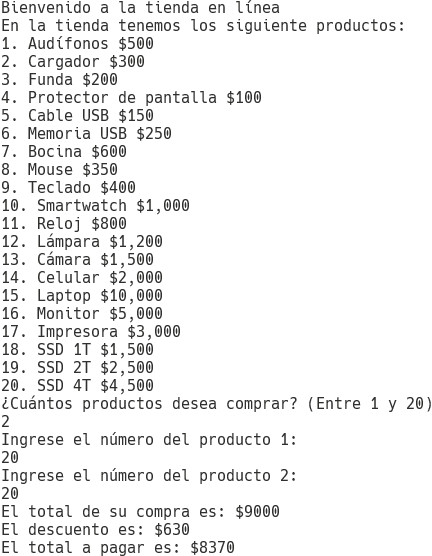
\includegraphics[width=0.4\columnwidth, center]{P1.png}
  % \end{figure}

  
  \subsection*{Problema 2}
  Del código de \textit{Snake} ubicado en:\url{https://github.com/LeonardoLed/POO/tree/main/TemaIII.HerenciayPolimorfismo/Prac3/Snake}

  Realice las siguientes modificaciones:
  \begin{itemize}
    \item Cambie las imágenes de la víbora y de la manzana por imágenes diferentes.
    \item Agregue un cuadrado de diálogo emergente que pregunte si quiere volver a jugar y si la respuesta es \textbf{sí} que se reinicie el juego y la respuesta es \textbf{no} se cierre la ventana.
    \item Cree una variable \textit{SCORE} donde se guarde el puntaje obtenido durante el juego y cuando se cierre el juego el puntaje final.
    \item Que la víbora al cruzar el final del \textit{JFrame} (cualquiera de los cuatro lados) no pierda el juego si no que aparezca del otro lado.
    \item Antes de iniciar el juego pregunte la velocidad del juego. Se manejarán tres
    velocidades:
    \begin{itemize}
      \item Lento (Babosa)
      \item Normal (Gusano)
      \item Rápido (Anaconda)
    \end{itemize}
    El juego se tendrá que comportar de la manera seleccionada.
  \end{itemize}

  \textbf{Explicación} \\
  Para cambiar las imágenes de la víbora y la manzana se necesitaban que los remplazos fueran de $10\times 10$ pixeles para mantener la misma escala en la ventana del juego. Las nuevas imágenes son las siguientes:

  \begin{figure}[ht]
    \centering
    \begin{minipage}[l]{0.3\columnwidth}
      
\includegraphics[width=\columnwidth, left]{dot.png}
      \caption*{Cuerpo}
    \end{minipage}
    \begin{minipage}[c]{0.3\columnwidth}
      
\includegraphics[width=\columnwidth, center]{head.png}
      \caption*{Cabeza}
    \end{minipage}
    \begin{minipage}[r]{0.25\columnwidth}
      
\includegraphics[width=\columnwidth, right]{apple.jpg}
      \caption*{Manzana}
    \end{minipage}
  \end{figure}

  Para agregar la opción de volver a jugar cuando se pierde el juego primero se para el \textit{timer} con el método \textit{stop()}, luego se utiliza la clase \textit{JOptionPane} y el método \textit{showConfirmDialog()} para desplegar una ventana con dos botones como se muestra en la siguiente imagen:

  \begin{figure}[ht]
    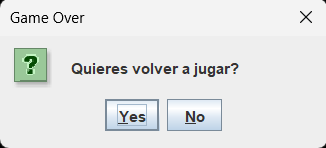
\includegraphics[width=0.75\columnwidth, center]{v1.png}
  \end{figure}

  Si se selecciona la opción \textit{Yes} la variable \textit{inGame} se reasigna a \textit{true}, la variable \textit{score} (que guarda la puntuación del jugador) se inicializa en 0 y se utiliza el método \textit{initGame()} para reiniciar el juego.

  Si se selecciona la opción \textit{No} se despliega una nueva ventana con el método \textit{showMessageDialog()} para mostrar el puntaje final y luego se termina la ejecución del juego.

  \begin{figure}[ht]
    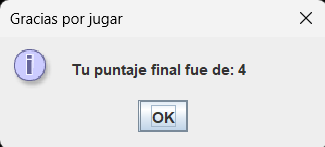
\includegraphics[width=0.75\columnwidth, center]{v2.png}
  \end{figure}  

  Para que el juego no termine cuando se choca con un borde de la ventana, es necesario cambiar las condiciones en el método \textit{checkCollision}. Si la cabeza de la víbora llega al borde superior o inferior, se cambia la posición de \textit{y} para aparecer del lado opuesto. Lo mismo ocurre con los bordes izquierdo y derecho pero cambiando la posición en \textit{x}.

  Finalmente, para jugar en 3 velocidades se creo un nuevo método llamado \textit{setSpeed()} que se llama al iniciar el juego. Primero se despliega una ventana en la que el usuario pueda seleccionar alguna de las 3 velocidades utilizando el método \textit{showInputDialog()} al que se le pasa como parámetro un arreglo de cadenas con las opciones disponibles.

  \begin{figure}[ht]
    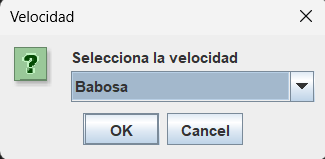
\includegraphics[width=0.75\columnwidth, center]{v3.png}
  \end{figure}
  
  Este método retorna la cadena que seleccionó el usuario y se guarda en una nueva variable para comprobar cual fue la selección. Para poder alterar la velocidad de movimiento de la víbora se cambió la constante \textit{DELAY} a una variable normal. En el caso de la velocidad ``Babosa'' se modificó el \textit{delay} a 160 para ir más lento y la velocidad ``Anaconda'' a 80 para ir más rápido.

  \textbf{Clase \textit{Snake}}
  \begin{lstlisting}
import java.awt.EventQueue;
import javax.swing.JFrame;

public class Snake extends JFrame {
  public Snake() {
    initUI();
  }

  private void initUI() {
    add(new Board());

    setResizable(false);
    pack();

    setTitle("Snake");
    setLocationRelativeTo(null);
    setDefaultCloseOperation(JFrame.EXIT_ON_CLOSE);
  }

  public static void main(String[] args) {
    EventQueue.invokeLater(() -> {
        JFrame ex = new Snake();
        ex.setVisible(true);
    });
  }
}
  \end{lstlisting}

  \textbf{Clase \textit{Board}}
  \begin{lstlisting}
import java.awt.Color;
import java.awt.Dimension;
import java.awt.Font;
import java.awt.FontMetrics;
import java.awt.Graphics;
import java.awt.Image;
import java.awt.Toolkit;

import java.awt.event.ActionEvent;
import java.awt.event.ActionListener;
import java.awt.event.KeyAdapter;
import java.awt.event.KeyEvent;

import javax.swing.ImageIcon;
import javax.swing.JOptionPane;
import javax.swing.JPanel;
import javax.swing.Timer;

// IMPLEMENTS -> INTERFACES
// EXTENDS -> CLASE PADRE (HERENCIA)

public class Board extends JPanel implements ActionListener {
  private final int WIDTH = 300;
  private final int HEIGHT = 300;
  private final int DOT_SIZE = 10;
  private final int ALL_DOTS = 900;
  private final int RAND_POS = 30;
  
  private final int x[] = new int[ALL_DOTS];
  private final int y[] = new int[ALL_DOTS];
  
  private int dots;
  private int apple_x;
  private int apple_y;
  private int score = 0;
  
  private boolean leftDirection = false;
  private boolean rigthDirection = true;
  private boolean upDirection = false;
  private boolean downDirection = false;
  private boolean inGame = true;

  private Image ball;
  private Image apple;
  private Image head;
  private Timer timer;
  private int delay = 120;
  
  private String[] speeds = { "Babosa", "Gusano", "Anaconda" };

  public Board() {
    initBoard();
  }

  // metodos de disenio

  private void initBoard() {
    addKeyListener(new TAdapter());
    setBackground(Color.black);
    setFocusable(true);

    setPreferredSize(new Dimension(WIDTH, HEIGHT));
    loadImages();
    setSpeed();
    initGame();
  }

  private void loadImages() {
    ImageIcon iid = new ImageIcon("img/dot.png");
    ball = iid.getImage();

    ImageIcon iia = new ImageIcon("img/apple.jpg");
    apple = iia.getImage();

    ImageIcon iih = new ImageIcon("img/head.png");
    head = iih.getImage();
  }

  private void setSpeed() {
    String speed = (String) JOptionPane.showInputDialog(
        this,
        "Selecciona la velocidad",
        "Velocidad",
        JOptionPane.QUESTION_MESSAGE,
        null,
        speeds,
        speeds[0]);

    if(speed.equals("Babosa"))
      delay = 160;
    else if(speed.equals("Anaconda"))
      delay = 80;
  }

  private void initGame() {
    dots = 3;

    for (int z = 0; z < dots; z++) {
      x[z] = 50 - z * 10;
      y[z] = 50;
    }

    locateApple();

    timer = new Timer(delay, this);
    timer.start();
  }

  @Override
  public void paintComponent(Graphics g) {
    super.paintComponent(g);
    doDrawing(g);
  }

  private void doDrawing(Graphics g) {
    if (inGame) {
      g.drawImage(apple, apple_x, apple_y, this);

      for (int z = 0; z < dots; z++) {
        if (z == 0) {
          g.drawImage(head, x[z], y[z], this);
        } else {
          g.drawImage(ball, x[z], y[z], this);
        }
      }
      Toolkit.getDefaultToolkit().sync();

      String msg = "Score: " + score;

      g.setColor(Color.white);
      g.setFont(new Font("Verdana", Font.BOLD, 20));
      g.drawString(msg, 20, 30);
    } else {
      gameOver(g);
    }
  }

  private void gameOver(Graphics g) {
    timer.stop();

    int n = JOptionPane.showConfirmDialog(
        this,
        "Quieres volver a jugar?",
        "Game Over",
        JOptionPane.YES_NO_OPTION);

    if (n == JOptionPane.YES_OPTION) {
      inGame = true;
      score = 0;
      initGame();
    } else {
      JOptionPane.showMessageDialog(
          this,
          "Tu puntaje final fue de: " + score,
          "Gracias por jugar",
          JOptionPane.INFORMATION_MESSAGE);

      System.exit(ABORT);
    }
  }

  private void move() {
    for (int z = dots; z > 0; z--) {
      x[z] = x[(z - 1)];
      y[z] = y[(z - 1)];
    }

    if (leftDirection) {
      x[0] -= DOT_SIZE;
    }
    if (rigthDirection) {
      x[0] += DOT_SIZE;
    }
    if (upDirection) {
      y[0] -= DOT_SIZE;
    }
    if (downDirection) {
      y[0] += DOT_SIZE;
    }

  }

  private void checkApple() {
    if ((x[0] == apple_x) && (y[0] == apple_y)) {
      dots++;
      score++;
      locateApple();
    }
  }

  private void locateApple() {
    int random = (int) (Math.random() * RAND_POS);
    apple_x = (random * DOT_SIZE);
    random = (int) (Math.random() * RAND_POS);
    apple_y = (random * DOT_SIZE);
  }

  private void checkCollision() {
    for (int z = dots; z > 0; z--) {
      if ((z > 4) && (x[0] == x[z]) && (y[0] == y[z])) {
        inGame = false;
      }
    }

    if (y[0] >= HEIGHT) {
      y[0] = 0;
    }
    if (y[0] < 0) {
      y[0] = HEIGHT;
    }
    if (x[0] >= WIDTH) {
      x[0] = 0;
    }
    if (x[0] < 0) {
      x[0] = WIDTH;
    }
  }

  @Override
  public void actionPerformed(ActionEvent e) {
    if (inGame) {
      checkApple();
      checkCollision();
      move();
    }
    repaint();
  }

  private class TAdapter extends KeyAdapter {
    @Override
    public void keyPressed(KeyEvent e) {
      int key = e.getKeyCode();

      if ((key == KeyEvent.VK_LEFT) && (!rigthDirection)) {
        leftDirection = true;
        upDirection = false;
        downDirection = false;
      }

      if ((key == KeyEvent.VK_RIGHT) && (!leftDirection)) {
        rigthDirection = true;
        upDirection = false;
        downDirection = false;
      }

      if ((key == KeyEvent.VK_UP) && (!downDirection)) {
        upDirection = true;
        rigthDirection = false;
        leftDirection = false;
      }

      if ((key == KeyEvent.VK_DOWN) && (!upDirection)) {
        downDirection = true;
        rigthDirection = false;
        leftDirection = false;
      }
    }
  }
}
  \end{lstlisting}

  \textbf{Ejecución}
  \begin{figure}[ht]
    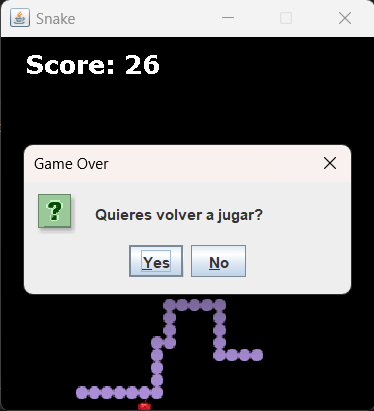
\includegraphics[width=0.8\columnwidth, center]{P2.png}
  \end{figure}

  \section*{Conclusiones}
  La programación orientada a objetos (POO) es un paradigma fundamental en la programación moderna que se basa en la creación de clases y objetos para modelar el mundo real de manera efectiva. A lo largo de este informe, hemos explorado los conceptos esenciales de la POO, que incluyen la creación de clases y objetos, el uso de métodos y constructores, la herencia, el polimorfismo y otros conceptos clave.

  La POO promueve el modularidad, la reutilización de código y la organización eficiente de sistemas complejos. Permite abordar problemas de manera más intuitiva al mapear objetos del mundo real a objetos de software

  \section*{Referencias}
  \small
  Solano, J. (2017, 20 enero). \textit{Manual de prácticas de Programación Orientada a Objetos}. Laboratorio de Computación Salas A y B. \url{http://lcp02.fi-b.unam.mx/} \\

  POO/TemaIII.HerenciayPolimorfismo/Prac3/Snake at main · LeonardoLed/POO. (n.d.). GitHub. \url{https://github.com/LeonardoLed/POO/tree/main/TemaIII.HerenciayPolimorfismo/Prac3}
\end{document}